\section{Data lifecycle}

\subsection{Data lifecycle management phases}
\noindent Many tools are available to help manage data throughout the research process; these can be categorized using data lifecyle management phases (illustrated below):

\begin{center}
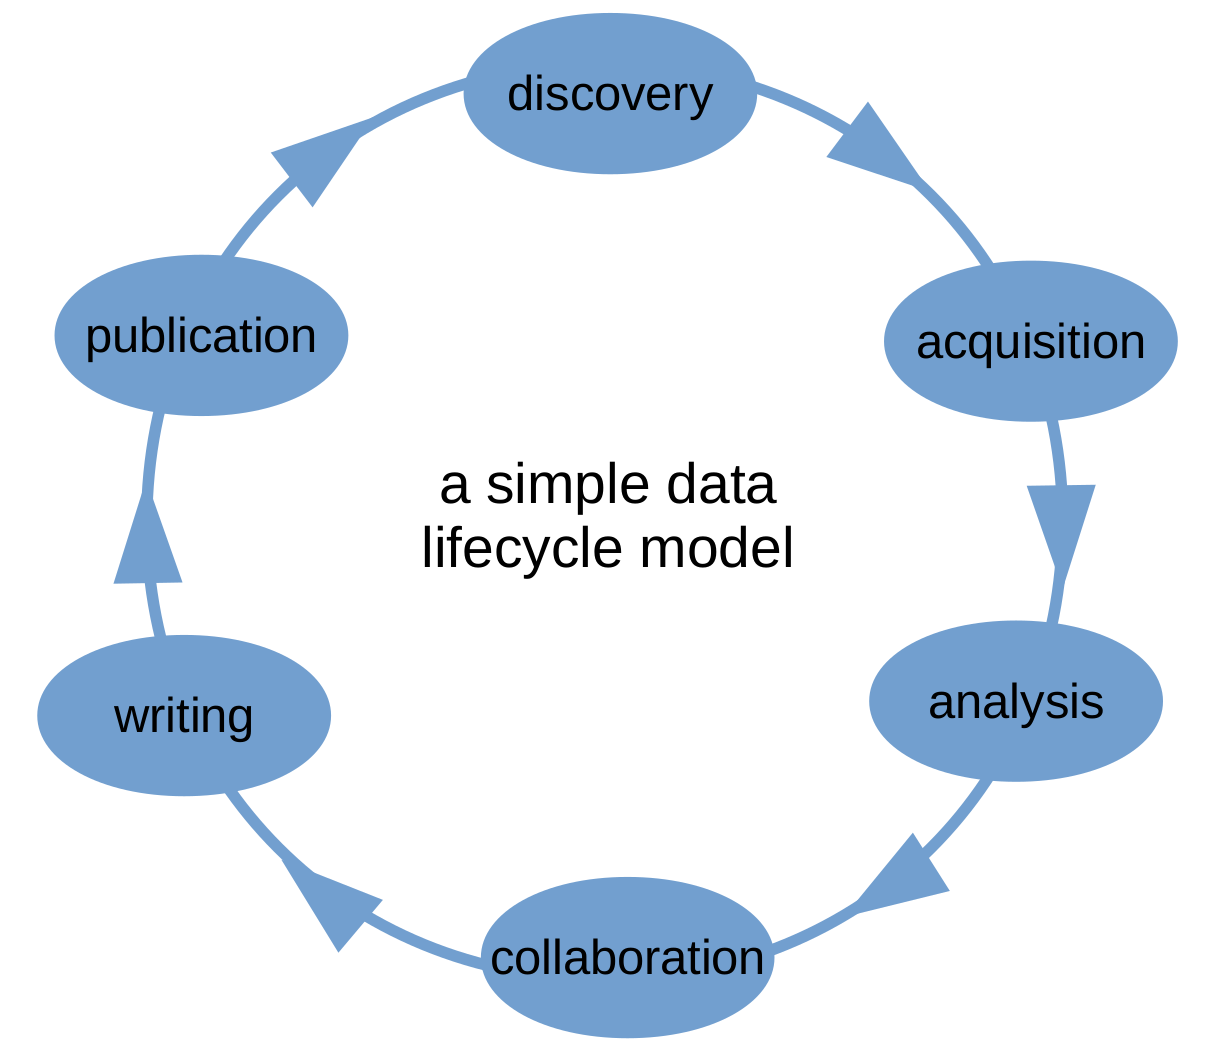
\includegraphics[width=0.55\textwidth]{./images/lifecycle.png}
\end{center}

\begin{enumerate}
\item \textbf{discovery:} find useful, technically and legally reusable datasets
\item \textbf{acquisition:} maximize the potential of your data, its visibility, and reproducibility by choosing from the beginning appropriated data and metadata formats. Anticipating will be crucial, knowing that afterwards it might be too late to do so.
\item \textbf{analysis:} analyze the data
\item \textbf{collaboration:} share your data and collaborate with your colleagues and partners (locally or worldwide)
\item \textbf{writing:} use comprehensive and collaborative paper writing tools
\item \textbf{publication:} deposit your datasets in visible and trusted data repositories
%\item \textbf{outreach:} enhance the visibility and discoverability of your datasets
%\item \textbf{assessment:} data quality evaluation
\end{enumerate}

\subsection{Data management planning tools}

Data management plans (DMP) are recognized as important means to produce data of good quality. DMPs are generally conceived from the beginning of research projects and updated throughout their duration. They aim to anticipate all data-related needs (such as storage capacities, collaborative tools, data licenses, data formats, metadata or description, sensitive data anonymization, etc.) and avoid any problems (lacunar data, data loss, data corruption, intellectual properties issues, storage, etc.).

\vspace{0.4cm}

\noindent \index{Data Management Plan!Online Tool}  \textsc{\href{http://dmponline.dcc.ac.uk/}{DMP Online}} (UK) and \textsc{\href{https://dmptool.org/}{DMP Tool}} (US) are free online tools assisting in the conception of DMPs. Both will guide the user through the essential questions that must be answered to manage your data. In addition, various funders' requirements are built in and can be used out of the box (e.g. DMP Online supports the Horizon 2020 guidelines)\cite{dmponline_dmponline_2015,dmptool_dmptool_2015}. 

\vspace{0.4cm}

\noindent \index{Data Management Plan!Howto} \textsc{\href{http://www.dcc.ac.uk/resources/how-guides/develop-data-plan}{How to Develop a Data Management}} is a more traditional guide describing the elaboration of a DMP \cite{digital_curation_centre_how_2015}.

\vspace{0.4cm}

\noindent \index{Data Management Policies!University of Edinburgh} \textsc{\href{http://ec.europa.eu/research/participants/data/ref/h2020/grants_manual/hi/oa_pilot/h2020-hi-oa-data-mgt_en.pdf}{Guidelines on Data Management in Horizon 2020}} are the official requirements to follow when appling to a Horizon 2020 project subject to the data pilot program \cite{european_comission_guidelines_2013}.

\vspace{0.4cm}

\subsection{Data policies}

\noindent \index{Data Management Policies!University of Edinburgh} \index{Data Management Policies!University of Oxford} \index{Data Management Policies!Humblodt University Berlin}  \index{Data Management Policies!University of Southampton} \index{Data Management Policies!University of Bath}The following institutional data policies, constitute together a good overview on this topic in Europe: \href{http://www.ed.ac.uk/schools-departments/information-services/about/policies-and-regulations/research-data-policy}{University of Edinburgh}, \href{http://researchdata.ox.ac.uk/university-of-oxford-policy-on-the-management-of-research-data-and-records/}{University of Oxford}, \href{https://www.cms.hu-berlin.de/de/ueberblick/projekte/dataman/policy/policy-en/rdm-eng-policy}{Humbolt University Berlin}, \href{http://www.calendar.soton.ac.uk/sectionIV/research-data-management.html}{University of Southampton} and \href{http://www.miss.manchester.ac.uk/?page_id=425}{University of Manchester} \cite{university_of_edinburgh_research_2015,university_of_oxford_university_2015,humboldt_university_berlin_research_2015,university_of_manchester_university_2015,university_of_southampton_university_2015}.

\section{Data management tools}

In this section data management tools are listed along each step of the data lifecycle. 

\subsection{Data discovery tools}

\subsubsection{Data repositories}

\label{ddtsec}

\noindent \index{Data Repositories!Re3data} \textsc{\href{http://re3data.org}{re3data.org}} is a registry of data repositories. This tool indexes over a thousand archives which are both subject specific and generalist and can be browsed by disciplines, available repositories features such as persistent identifiers support (e.g. DOIs, which play a crucial for guarantying access to datasets, as web links tend to break after a few years), and other important information such as data licenses availability, standards and policies \cite{re3data_re3data.org_2015}.

\vspace{0.4cm}

\noindent \index{Recommended!Data Repositories} \index{Data Repositories!Recommended Repositories} \textsc{\href{http://www.nature.com/sdata/data-policies/repositories}{Nature's Recommended Data Repositories}} is a set of disciplinary repositories covering the following fields: Biological sciences; Health sciences; Chemistry; Earth and environmental sciences; Physics, astrophysics \& astronomy; Social sciences; and General science \cite{nature_publishing_group_recommended_2014}.

\vspace{0.4cm}

\noindent \index{Data Repositories!Zenodo} \textsc{\href{http://zenodo.org}{Zenodo}} \cite{zenodo_zenodo_2015}, \index{Data Repositories!Dryad} \textsc{\href{http://datadryad.org/}{dryad}} \cite{dryad_dryad_2015}  and \index{Data Repositories!Figshare} \textsc{\href{http://figshare.com/}{figshare}} \cite{figshare_figshare_2015} are state of the art general-purpose data repositories. Zenodo is made available by Cern and OpenAire and is free for any researcher publishing his or her data openly. Dryad is a curated repository, maintained by a non profit organization. Figshare belongs to a for profit company, the MacMillan group, which also owns the Nature Publishing Group.


\subsubsection{Data papers and data  journals}

\index{Data Journals!Data Papers} Data papers are publications describing datasets. In other words, they constitute peer-reviewed searchable metadata, and they can be used to find or highlight datasets. Data papers can be found in pure data journals, or in journals mixed with traditional scholarly publications. An important point, is that these papers may be found through classical scholarly search engines. In addition, the following resources can help you find multi-disciplinary datajournals and data papers:
\begin{itemize}
\item \index{Data Journals!Dryad's Data Journals List} \href{http://wiki.datadryad.org/Journal_instructions#Examples_of_journal_data_policies}{Dryad's examples of journal data policies} lists journals that require data archiving and journals with data policies \cite{dryad_journal_2015}
\item \index{Data Journals!Trac's atadData Journals List} Trac's multidisciplinary \href{http://proj.badc.rl.ac.uk/preparde/blog/DataJournalsList}{data journals list}\cite{trac_blog:_2013}
\item \index{Data Journals!Nature's Scientific Data} Nature Publishing Group's \href{http://www.nature.com/sdata/}{scientific data website} \cite{nature_publishing_group_scientific_2015}
\item DataShare's \href{https://www.wiki.ed.ac.uk/display/datashare/Sources+of+dataset+peer+review}{sources of dataset peer review} list of data journals \cite{datashare_sources_2015}
\item \index{Data Journals!GigaScience} \href{http://www.gigasciencejournal.com/}{GigaScience} \cite{gigascience_gigascience_2015}
\end{itemize}

Some discipline specific data journals exist too, for example:
\begin{itemize}
\item \index{Data Journals!Earth System Sicience Data} \index{Data Journals!Geoscience Data Journal} Wiley's \href{http://onlinelibrary.wiley.com/journal/10.1002/%28ISSN%292049-6060}{Geoscience Data Journal} and \href{http://www.earth-system-science-data.net/}{Earth System Science Data} \cite{earth_system_science_data_essd_2015}
\item \index{Data Journals!Open Health Data} UpMetaJournal's \href{http://openhealthdata.metajnl.com/}{Open Health Data} \cite{upmetajournals_open_2015}
\item \index{Data Journals!Biodiversity Data Journal} Pensoft's \href{http://biodiversitydatajournal.com/}{Biodiversity Data Journal} \cite{pensoft_biodiversity_2015}
\item \index{Data Journals!Archaeology Data Journal} UpMetaJournal's \href{http://openarchaeologydata.metajnl.com/}{Journal of open archaeology data} \cite{upmetajournals_journal_2015}
\end{itemize}

\noindent In addition, a list of \textsc{\href{http://datadryad.org/pages/jdap}{Journals Data Policies}} compiled by Dryad may be of interest \cite{dryad_joint_2014}.

\subsection{Data acquisition, format and description}

In order to make the most out of your research data, it is important to use appropriated data and metadata standards. This has to be thought through at the beginning of the project and in any case before data acquisition. Indeed, it is often to late to correct, complete or correct data after the project is well started. Using good data and metadata standard help collecting coherent data and avoid missing some points. In addition, badly described data will not be re-usable by others at all, nor will it be easy to find. A standard and open data format will allow more people to access and re-use a dataset because of its good compatibility across software and platforms. Finally, open standards will maximize the chances to access your results in the future because they are supported longer.


\subsubsection{Data acquisition}

\noindent \index{Software!Science Exchange} \textsc{\href{http://scienceexchange.com}{ScienceExchange}} is a platform where scientists can order data for specific experiments (including from their own design): it is an on-line scientific experiment marketplace \cite{scienceexchange_science_2015}.

\vspace{0.4cm}

\noindent \index{Software!RopenSci} \textsc{\href{http://ropensci.org}{RopenSci}} offers packages providing an easy access to data repositories through the \href{http://r-project.org}{R statistical programming environment}. R is a free software available on all platforms (Windows, Mac, Linux). These packages cover data access in the following domains: primary data, full-text of journal articles, altmetrics, data-publication, reproducibility and data visualization. Many other data analysis R packages are available through \href{http://cran.r-project.org/}{CRAN} \cite{ropensci.org_ropensci_2015,r_project_r:_2015}.

\subsubsection{Data formats}

\noindent A directory of \index{Recommended!Data Formats} \index{Data Formats!Recommended Data Formats} \textsc{\href{http://www.digitalpreservation.gov/formats/}{Recommended Data Formats}} is maintained by the US Library of Congress. It covers the following categories: still images, sounds, moving images, textual documents, web archives, datasets, geospatial data as well as generic data \cite{libraryofcongress_sustainability_2015}.

\vspace{0.4cm}

\noindent The \index{Data Formats!Data Type Registry} \textsc{\href{http://www.typeregistry.org/registrar/}{DataTypeRegistry}} is a generic open source data type description platform. It allows in particular to combine already described units or data types to create new ones. Data types are labeled with unique identifiers. In addition to a web interface an automated access is allowed through the API \cite{datatyperegistry_data_2015}.

\vspace{0.4cm}

\noindent \index{Recommended!HDF5} \index{Data Formats!HDF5} \textsc{\href{https://www.hdfgroup.org/HDF5/}{HDF5}} ``is a data model, library, and file format for storing and managing data. It supports an unlimited variety of datatypes, and is designed for flexible and efficient I/O and for high volume and complex data. HDF5 is portable and is extensible, allowing applications to evolve in their use of HDF5. The HDF5 Technology suite includes tools and applications for managing, manipulating, viewing, and analyzing data in the HDF5 format'' \cite{hdf_group_hdf5_2015}. HDF5 is supported form within many environments such as Matlab, Octave, Python (H5py, PyTables), GNU-R, Java, C++, Fortran and Mathematica.

\vspace{0.4cm}

\noindent The \index{Data Formats!Structured Query Language (SQL)} \textsc{\href{https://en.wikipedia.org/wiki/SQL}{Structured Query Language (SQL)}} ``a special-purpose programming language designed for managing data held in a relational database management system (RDBMS)''\cite{wikipedia_sql_2015}. SQL is well suited to store and share relational data. RDBMS are a great help in maintaining dateset's coherence and enforce data constraints. Several multi-platform open source RDBMS are available, such as \href{https://mariadb.org/}{MariaDB} (MySQL) \cite{mariadb_mariadb_2015} or \href{http://www.postgresql.org/}{PosgreSQL} \cite{postgresql_postgresql:_2015}.

\vspace{0.4cm}

\noindent The \index{Data Formats!Semantic Web (RDF)} \textsc{\href{http://www.w3.org/RDF/}{Semantic Web}} Resource Description Format (RDF) ``is a standard model data interchange on the Web''\cite{w3c_rdf_2014}. RDF is a very general format and may be used to encode most types of data. A significant advantage of RDF over other data formats resides in its interoperablity capabilities with other datasources, allowing to extend analyses beyond given datasets by connecting them to other data sources. In practice, this is done using the SPARQL query language on \href{http://www.w3.org/wiki/LargeTripleStores}{triple stores} such as Virtuoso, Jena or 4store.

\vspace{0.4cm}

\noindent Sometimes, a simple but clear datasets  \index{Data Formats!Naming Convention} \textsc{Naming Convention} can help a lot. Consider e.g. the pattern: Project-Institution-Group-DataSetName-Version-YYYYMMDD.DataFormat, which could in practice become something like FictiveProject-UniversityX-SignalProcessingLab-SolarIntensity-Version2.3-20151131.csv .

\subsubsection{Metadata formats}

\noindent \index{Metadata Formats!DublinCore} \textsc{\href{http://dublincore.org/documents/dces/}{DublinCore}} is a vocabulary consisting of only 15 basic elements, such as Creator, Title, Date, Description, Format, Rights, or Subject \cite{dublincore_dublin_3013}. It is not specifically designed for dataset description, but widely used in scholarly communication. For that reason, it is a minimalist solution, and we recommend one of the solutions listed below instead. 

\vspace{0.4cm}

\noindent \index{Metadata Formats!DataCite} \textsc{\href{https://schema.datacite.org/}{DataCite Metadata Schema}} is a standard designed with datasets in mind, and hence more adapted then DublinCore mentioned just above. For example, GeoLocation, ReserarchGroups, Collections, Videos or Workflows have their own specific resource types \cite{datacite_datacite_2015}.

\vspace{0.4cm}

\noindent A directory of \index{Recommended!Metadata Formats} \index{Metadata Formats!Directory} \textsc{\href{http://rd-alliance.github.io/metadata-directory/}{Recommended Metadata Formats}} is available in this open source collaborative platform. They are indexed by discipline, extensions, associated tools and associated use cases. General available subject categories are Art and Humanities, Engineering, Life Sciences, Physical Sciences and Mathematics, Social and Behavioral Sciences and General Research Data. Dozens of subcategories are also available \cite{metadatadirectory_metadata_2015}.

\vspace{0.4cm}

\noindent The \index{Metadata Formats!Semantic Web (OWL)} \textsc{\href{http://www.w3.org/RDF/}{Semantic Web }} Resource Description Format (RDF) ``is a standard model data interchange on the Web''\cite{w3c_rdf_2014}. RDF is a very general format and may be used to encode most types of data. Indeed, many \href{http://www.w3.org/2001/sw/wiki/OWL}{OWL} \cite{w3c_owl_2009} RDF based ontologies exist. Ontologies are ``formal naming and definition of types, properties and interrelationship'' of data \cite{wikipedia_ontology_2015}.

\vspace{0.4cm}

\index{Metadata Formats!UML} \textsc{\href{http://www.uml.org/}{Unified Modeling Language (UML)}} is a complete modeling language. The class diagrams are particularly useful to describe data structures \cite{uml.org_unified_2015}.

\vspace{0.4cm}

\noindent Sometimes, a simple but clear \index{Metadata Formats!Textual description} \textsc{Textual Description} of a dataset can help a lot (even its own creator in the future). For instance, if it is not explicit in the dataset, it is a means to describe how, when, where and with what device the data has been gathered. In addition, the meaning of the labels (e.g. the column headers) are generally of interest, and so are the physical units and their accuracy.

\subsection{Data analysis tools}

\label{daanto}

\subsubsection{Statistical data analysis tools}
\noindent \index{Software!R Project} The \textsc{\href{http://r-project.org}{R statistical programming environment}} is a free software available on all platforms (Windows, Mac, Linux). In addition, \href{http://ropensci.org}{RopenSci} offers packages allowing an easy access to data repositories through R. These packages cover data access in the following domains: primary data, full-text of journal articles, altmetrics, data-publication, reproducibility and data visualization. Many other data analysis R packages are available through \href{http://cran.r-project.org/}{CRAN} \cite{ropensci.org_ropensci_2015,r_project_r:_2015}.

\vspace{0.4cm}

\noindent \index{Software!SPSS} \textsc{\href{http://www.ibm.com/software/analytics/spss/}{SPSS}} is a tool for statistical analysis, popular in social sicences. It is a proprietary software available on all platforms (Windows, Mac, Linux). IBM SPSS Modeler is a companion product for data mining. \index{Software!PSPP} \textsc{\href{http://www.gnu.org/software/pspp/}{PSPP}} is an open source multi-platform SPSS clone. Many SPSS features are supported by PSPP \cite{ibm_ibm_2015,gnu_pspp_2015}.

\subsubsection{Scientific and general data analysis tools}
\noindent \index{Software!Matlab} \textsc{\href{https://ch.mathworks.com/products/matlab/}{Matlab}} is an high-level interactive environment specializing in engineering and scientific computations. Matlab is a proprietary software available on all platforms (Windows, Mac, Linux). It covers in particular signal and image processing, communications, and control systems. \index{Software!Octave} \textsc{\href{http://www.gnu.org/software/octave/}{GNU Octave}} is an open source multi-platform Matlab clone. Many Matlab features are supported by Octave \cite{gnu_gnu_2015,mathworks_matlab_2015}.

\vspace{0.4cm}

\noindent \index{Software!NumPy} \index{Software!Python} \textsc{\href{http://www.numpy.org}{NumPy}} is a scientific package for computing with \href{http://www.python.org/}{Python}. It is a free software available on all platforms (Windows, Mac, Linux). It may be completed with many other scientific packages that may be found in the \href{https://pypi.python.org/pypi}{Python Package Index (PyPI)}, \href{http://pydata.org/downloads/}{PyData} and/or \href{http://www.scipy.org/}{SciPy}. For example: Matplotlib (plotting), Sympy (symbolic mathematics), Pandas (data structures and analysis) \cite{numpy_numpy_2015,python_software_foundation_python.org_2015,pydata_pydata.org_2015}.

\subsubsection{Mathematical symbolic analysis tools}

\noindent \index{Software!Mathematica}  \textsc{\href{http://www.wolfram.com/mathematica/}{Mathematica}} and \index{Software!Maple} \textsc{\href{http://www.maplesoft.com/products/maple/}{Maple}} are both mathematics, scientific and engineering oriented computing environments. They are based on symbolic mathematics and their interfaces take the form of interactive documents. Both are proprietary multi-platform software \cite{maplesoft_maple_2015,wolfram_wolfram_2015}.


\subsection{Active data collaboration tools}

\subsubsection{Versioning}

\noindent Versioning is a crucial tool for reproducible research, especially in the context of data and computer code: reproducing results generally requires at least to be able to combine the exact version of a dataset and the matching version of the computer code that exploits it. It is however not always sufficient, as in some cases the computing environment and hardware may also play a part in reproducibility.

\vspace{0.4cm}

\noindent \index{Software!Git} \textsc{\href{https://git-scm.com/}{Git}} is a free multi-platform revision control system. Git allows to track versions of large textual datasets (such as computer code or \LaTeX documents), and enables to restore, compare and merge files across their various branches and versions. Git supports decentralized work and nonlinear workflows. \index{Software!GitHUB} \textsc{\href{https://github.com/}{GitHUB}} is a git hosting platform, including open and private repositories, and provides additional features \cite{_git_2015,github_github_2015}. Many institutions offer their own Git server and include access rights (e.g. the \href{http://git.epfl.ch}{EPFL Git server}). Using an institutional server generally ensures that your data is safely stored and it avoids data leaks\index{EPFL!Git}. 

\subsubsection{File sharing}

\noindent The \textsc{institutional file share} is usually a good option if you are not working with external people.  Using an institutional server generally ensures that your data is safely stored and it avoids data leaks. For example, at EPFL\index{EPFL!Institutional File Share}, the default on-line storage can be monitored from \href{http://mynas.epfl.ch}{the MyNAS Web interface}, in which it is possible to request more space and find the access configuration for each operating system. In addition, the EPFL-IT services offers a range of storage options, depending on the quantity and the access modalities required for your data. For more information please contact \href{mailto:1234@epfl.ch}{1234@epfl.ch}. 

\vspace{0.4cm}

\noindent \label{ownCloud} \index{Software!OwnCloud} \textsc{\href{http://owncloud.org}{ownCloud}} is a free software: it synchronizes and shares data on several computers (supported systems: Windows, Linux, Mac, Android and iOS). OwnCloud functionality may be extended through many plugins such as calender share, collaborative editing, music player, pictures galleries, password storage, and so on. Intuitions often offer an ownCloud instance to their members. Using an institutional server generally ensures that your data is safely stored and avoids data leaks\index{EPFL!OwnCloud}. For example, EPFL members have free access to \textsc{\href{http://drive.switch.ch}{SwitchDrive}}, an instance of ownCloud opened to most Swiss universites, and therefore, ideal for sharing data among the national academic community\cite{owncloud_owncloud.org_2015,switchdrive_switchdrive_2015}. If an institutional instance is not available or unsuitable for your  needs, many ownCloud \href{https://owncloud.org/providers/}{providers} are available\cite{owncloud.org_owncloud_2015}, including some in Switzerland, e.g \href{https://woelkli.com}{Woelkli.com}\cite{woelkli_secure_2015}.   

\vspace{0.4cm}

\noindent \index{Software!Git-annex} \index{Software!Git-annex Assistant} \textsc{\href{http://git-annex.branchable.com/}{git-annex}} is an extension of Git, the versioning software described in the previous section. \textit{Per se} Git is not well suited to manage non-textual (binary) files. This tool extends Git in that regard, and comes with the git-annex assistant, allowing to create an easy to use decentralized file share. In other words, this is comparable sharing file via ownCloud, however without the need for a central server \cite{git-annex_git-annex_2015}.

\subsubsection{Graphs}

\noindent \index{Software!Plotly} \textsc{\href{https://plot.ly}{Plotly}} is a collaborative ``suite of data visualistion and collaboration tools for engineers and data scientists'' \cite{plot.ly_plotly_2015}.

\vspace{0.4cm}

\noindent \index{Software!Dia} \textsc{\href{https://wiki.gnome.org/Apps/Dia/}{Dia}} is a multiplatform open source diagram editor that supports among others Unified Modeling Language (UML) formalism \cite{gnu_dia_2015}.

\vspace{0.4cm}

\noindent \index{Software!Graphviz} \textsc{\href{http://www.graphviz.org/}{Graphviz}} ``Graphviz is open source graph visualization software. Graph visualization is a way of representing structural information as diagrams of abstract graphs and networks. It has important applications in networking, bioinformatics,  software engineering, database and web design, machine learning, and in visual interfaces for other technical domains'' \cite{graphviz_graph_2015}.

\subsubsection{Geodata}

\noindent \index{Software!QGIS} \textsc{\href{http://www.qgis.org/en/site/}{QGIS}} is a free multi-platform Geographic Information System (GIS) software with data editing, analysis and viewing functionality \cite{qgis.org_qgis_2015}.

\subsubsection{3D} 

\noindent \index{Software!ParaView} \textsc{\href{http://www.paraview.org/}{ParaView}}  ``is an open-source, multi-platform data analysis and visualization application. ParaView users can quickly build visualizations to analyze their data using qualitative and quantitative techniques. The data exploration can be done interactively in 3D or programmatically using ParaView’s batch processing capabilities. ParaView was developed to analyze extremely large datasets using distributed memory computing resources'' \cite{paraview.org_paraview_2015}.

\vspace{0.4cm}

\noindent \index{Software!MeshLab} \textsc{\href{http://meshlab.sourceforge.net/}{MeshLab}}  ``MeshLab is an open source, portable, and extensible system for the processing and editing of unstructured 3D triangular meshes'' \cite{meshlab.sf.net_meshlab_2015}. MeshLab can convert mesh files to STereoLithography (STL) files, widely used by 3D applications.


\subsubsection{Papers and annotations}

\label{angrpatd}

\noindent \index{Software!Authorea} \textsc{\href{https://www.authorea.com/}{Authorea}} is collaborative \LaTeX based writing tool: it handles group authoring. It supports text, images, mathematical formulas, computer code, bibliographic reference management, citation and bibliography, footnotes, commentaries, iPhython Notebooks, and many other features.  \index{Software!OverLeaf} A third alternative to Atlas and Authorea is \textsc{\href{https://www.overleaf.com/}{OverLeaf}} \cite{authorea_authorea:_2015,oreilley_getting-started--atlas_2015}.

\vspace{0.4cm}

\noindent \index{Software!Atlas} \href{http://atlas.oreiley.com}{Atlas} is another collaborative writing tool similar to Authorea, but WYSIWYG (WYSIWYG: what you see is what you get, in practice similar to a classical word processing application). The \href{https://github.com/oreillymedia/Getting-Started-with-Atlas}{Atlas platform} is a free software and could therefore be installed locally on your server or more generally at your institution \cite{oreilly_atlas_2015,authorea_authorea:_2015,oreilley_getting-started--atlas_2015}.

\vspace{0.4cm}

\noindent \index{Software!Hypothseis} \textsc{\href{https://hypothes.is}{Hypothesis}} is collaborative annotation tool, with which you can take personal notes, discuss, collaborate and organize your research \cite{hypothes.is_hypothesis_2015}.

\vspace{0.4cm}

\noindent \index{Software!OwnCloud} \textsc{\href{http://owncloud.org}{ownCloud}} is a collaborative software, particularly useful for file sharing (see section \ref{ownCloud}). In addition, many plugins, such as text editor with real-time \href{https://www.youtube.com/watch?v=xsqSLeppxm0}{collaborative editing} are available \cite{owncloud_owncloud.org_2015}. 

%
% Think about adding : etherpad/framapad, abiword
%

\subsubsection{Reference management and sharing}

Reference management is generally integrated in collaborative authoring tools (e.g. Authorea, Atlas, Overleaf), which were discussed in the previous section.

\vspace{0.4cm}

\noindent \index{Software!Zotero} \textsc{\href{https://www.zotero.org/}{Zotero}} is a free mutltiplatform reference management software: it manages bibliographic references and associated research materials (PDF files, Web pages captures, etc.). A specificity of Zotero is its integration with Web browsers, which allows to naturally capture research materials and references in one click while surfing. The software is extensible via plugins, in particular writing tools for citation and bibliography management. The tool boasts an excellent integration with Libre Office, Open Office, and Neo Office Microsoft Word, and BibTex is supported. The Zotero social and collaborative features enable the synchronization of bibliographies among public or private groups. Ressource annotations are shared as well. Zotero does not require the users to upload any data to its servers \cite{zotero.org_zotero_2015}.

\vspace{0.4cm}

\noindent \index{Software!Mendeley} \textsc{\href{https://www.mendeley.com/}{Mendeley}} is another multiplatform desktop reference management software and an online social researcher network. Contrarily to Zotero, all basic metadata is sent to its servers and this cannot be turned off. Mendeley is a proprietary software bolonging to Elsevier \cite{mendeley.com_mendeley_2015}. 

\subsubsection{Sientific workflows and laboratory management}

\noindent \index{Software!MyExperiment} \textsc{\href{http://www.myexperiment.org}{myExperiment}} ``is a social website for sharing [...] scientific workflows [...]'' and integrates many tools such as Taverna and Bioclipse \cite{myexperiment_myexperiment_2014,myexperiment.org_myexperiment_2015}.

\vspace{0.4cm}

\noindent \index{Software!AiiDA} \index{EPFL!AiiDA} \textsc{\href{http://www.aiida.net/}{AiiDA}}, the Automated Interactive Infrastructure and Database for Computational is a ``flexible and scalable informatics' infrastructure to manage, preserve, and disseminate the simulations, data, and workflows of modern-day computational science. Able to store the full provenance of each object, and based on a tailored database built for efficient data mining of heterogeneous results, AiiDA gives the user the ability to interact seamlessly with any number of remote HPC resources and codes, thanks to its flexible plugin interface and workflow engine for the automation of complex sequences of simulations'' \cite{aiida.net_aiida_2015}. This tool is developed at EPFL. AiiDA's core is free software, some of its plugins are licensed for non-commercial use \cite{pizzi_aiida:_2015}.

\vspace{0.4cm}

\noindent \index{Software!Taverna} \index{Software!Pegasus} \textsc{\href{http://pegasus.isi.edu/}{Pegasus}} and \textsc{\href{http://www.taverna.org.uk/}{Taverna}} are open source workflow management systems, both able to execute applications \cite{pegasus_pegasus_2015,taverna_taverna_2015}.

\vspace{0.4cm}

\noindent \index{Software!Kepler} \textsc{\href{https://kepler-project.org/}{Kepler}} is a free software system for designing, executing, reusing, evolving, archiving, and sharing scientific workflows \cite{kepler-project.org_kepler_2015,kepler-project.org_kepler_2015-1}.

\vspace{0.4cm}

\noindent \index{Software!LIMS} \index{Software!SLIMS} \index{Software!OpenBIS} \textsc{\href{https://en.wikipedia.org/wiki/Laboratory_information_management_system}{Laboratory Information Management Systems}} are software that take modern laboratory operations in charge. Their features often include workflow management, data tracking, sample tracking, data exchange interfaces and enterprise resource planning \cite{wikipedia_laboratory_2015}. For example, at EPFL several labs use the \href{http://sv-it.epfl.ch/slims}{SLIMS} software and ETHZ is developing an open source tool: \href{http://www.cisd.ethz.ch/software/openBIS}{openBIS} \cite{ethz_eth_2015,epfl_lsis_2015}.


\subsection{Data publication tools}

\subsubsection{Data repositories}

Data repositories are listed in section \ref{ddtsec}, page \pageref{ddtsec}.

\subsubsection{Interactive publications}

Interactive publications are a new generation of publications: in addition to the iPython Notebooks  discussed just below, Maple and Mathematica use the concept interactive publication too. These software are however more mathematics-oriented (see section \ref{daanto} on page \pageref{daanto}).

\vspace{0.4cm}

\index{Software!iPython Notebooks} \textsc{\href{http://ipython.org/notebook.html}{iPython Notebooks}} (IPYNB) are interactive publications making use of the Python language. Hence, these are based on free and multiplatform software. Such notebooks have two advantages in academia: they promote research reproducibility (because they constitute an excellent way to comment the code, run on all platforms and require only free software) and are excellent pedagogical tools. A student may easily play with the code illustrating a concept, for example he or she can change parameters to get a practical understanding of theories and algorithms. Practically, in addition to the interpreted-code parts, IPYNB can be structured using various header-levels, rich text (markdown), and mathematical formulas (\LaTeX). Since they are Python based, these notebook can take advantage of many scientific packages that may be found in the \href{https://pypi.python.org/pypi}{Python Package Index (PyPI)}, \href{http://pydata.org/downloads/}{PyData} and/or \href{http://www.scipy.org/}{SciPy}. For example: NumPy (numeric analysis), Matplotlib (plotting), Sympy (symbolic mathematics), Pandas (data structures and analysis) \cite{numpy_numpy_2015,python_software_foundation_python.org_2015}. In addition, iPython notebooks may be shared or hosted through Web based tools such as the collaborative writing platform Authorea (see section \ref{angrpatd} page \pageref{angrpatd}) or \href{https://wakari.io/}{Wakari.io} \cite{wikipedia_ipython_2015,ipython.org_ipython_2015}.

\subsubsection{Data licenses and Laws}

\paragraph{Personal Data Protection Laws}

~

\noindent \index{Laws!EU} The \textsc{European Union} has a personal data legal protection framework. An significant part of this is \textsc{\href{http://eur-lex.europa.eu/LexUriServ/LexUriServ.do?uri=CELEX:31995L0046:en:HTML}{Directive 95/46/EC}} \cite{eurlex_9546ec_1995}, which will probably be superseded by the \textsc{\href{https://en.wikipedia.org/wiki/General_Data_Protection_Regulation}{General Data Protection Directive (GDPR)}} \cite{wikipedia_general_2015}.

\vspace{0.4cm}

\noindent \index{Laws!CH} The \textsc{Switzerland} has a personal data legal protection framework. An significant part of this is \textsc{\href{https://www.admin.ch/opc/fr/classified-compilation/19920153/}{Loi fédérale sur la protection des données (LPD)}} \cite{admin.ch_rs_1992} .


\paragraph{Text and multimedia licenses}

~

\noindent \index{Licences!Creative Commons By} \textsc{\href{https://creativecommons.org/}{Creative Commons BY}} licenses enable to choose exactly what is allowed to do with your text and multimedia documents. In addition to the CC0 (see below), the CC-BY offers 6 variants\cite{creativecommons.org_creative_2015}:
\begin{itemize}
\item
\includegraphics[width=15mm]{./images/CC-By_88x31.png} (Attribution : CC-By) ``lets others distribute, remix, tweak, and build upon your work, even commercially, as long as they credit you for the original creation. This is the most accommodating of licenses offered.''
\item
\includegraphics[width=15mm]{./images/CC-By-SA_88x31.png} (Attribution-ShareAlike) ``lets others remix, tweak, and build upon your work even for commercial purposes, as long as they credit you and license their new creations under the identical terms. [...] All new works based on yours will carry the same license, so any derivatives will also allow commercial use.''
\item
\includegraphics[width=15mm]{./images/CC-By-ND_88x31.png} (Attribution-NoDerivs) ``This license allows for redistribution, commercial and non-commercial, as long as it is passed along unchanged and in whole, with credit to you.''
\item
\includegraphics[width=15mm]{./images/CC-By-NC_88x31.png} (Attribution-NonCommercial) ``lets others remix, tweak, and build upon your work non-commercially, and although their new works must also acknowledge you and be non-commercial, they don’t have to license their derivative works on the same terms.''
\item
\includegraphics[width=15mm]{./images/CC-By-NC-SA_88x31.png} (Attribution-NonCommercial-ShareAlike) ``lets others remix, tweak, and build upon your work non-commercially, as long as they credit you and license their new creations under the identical terms.''
\item
\includegraphics[width=15mm]{./images/CC-By-NC-ND_88x31.png} (Attribution-NonCommercial-NoDerivs) ``This license is the most restrictive of [the Creative Commons] six main licenses, only allowing others to download your works and share them with others as long as they credit you, but they can’t change them in any way or use them commercially.''
\end{itemize}


\vspace{0.4cm}

\noindent \label{lcc0} \index{Licences!Creative Commons Zero} \textsc{\href{https://creativecommons.org/}{Creative Commons Zero}} 
\includegraphics[width=15mm]{./images/CC0-88x31.png}, contrarily to CC-By the ``CC0 enables scientists, educators, artists and other creators and owners of copyright- or database-protected content to waive those interests in their works and thereby place them as completely as possible in the public domain, so that others may freely build upon, enhance and reuse the works for any purposes without restriction under copyright or database law'' \cite{creativecommons.org_creative_2015}.

\paragraph{Computer code licenses}

~

\noindent \index{Licences!GNU General Public Licence (GPL)} \textsc{\href{http://www.gnu.org/licenses/gpl.html}{GNU General Public licence (GPL)}} 
\includegraphics[width=15mm]{./images/gplv3-127x51.png} is to software what the Creative Commons Attribution-ShareAlike is to documents. It is the typical free software copyleft license and guarantees four freedoms to the users \cite{fsf_gpl_2105}:
\begin{itemize}
\item the freedom to use the software for any purpose,
\item the freedom to change the software to suit your needs,
\item the freedom to share the software with your friends and neighbors, and
\item the freedom to share the changes you make.
\end{itemize}

Many licences are compatible with GPLv3, notably: Apache Licence 2.0, Artistic Licence 2.0, Berkley Database Licence, Modified BSD License, Boost Software License, CeCILL, CreativeCommons Zero, Educationnal Community Licence, AGLP, LGPL, IBM Public Licence, Intel Open source License, ISC License, MIT License / X11 License, Python Software Lisence, W3C Software Notice and LicenseXFree86 Lisence, zlib/libpng License and Zope Public Lisence.  \cite{wikipedia_comparison_2015}

\vspace{0.4cm}

\noindent \index{Licences!GNU Lesser General Public Licence (LGPL)} \textsc{\href{http://www.gnu.org/licenses/lgpl.html}{GNU Lesser General Public licence (LGPL)}} ``The GNU Project has two principal licenses to use for libraries. One is the GNU Lesser GPL; the other is the ordinary GNU GPL. The choice of license makes a big difference: using the Lesser GPL permits use of the library in proprietary programs; using the ordinary GPL for a library makes it available only for free programs'' \cite{fsf_lgpl_2015}.

\vspace{0.4cm}

\noindent \index{Licences!GNU Affero General Public Licence (AGPL)} \textsc{\href{http://www.gnu.org/licenses/agpl.html}{GNU Affero Genreal Public licence (AGPL)}} ``The GNU Affero General Public License is a modified version of the ordinary GNU GPL version 3. It has one added requirement: if you run a modified program on a server and let other users communicate with it there, your server must also allow them to download the source code corresponding to the modified version running there. The purpose of the GNU Affero GPL is to prevent a problem that affects developers of free programs that are often used on servers'' \cite{fsf_agpl_2015}.

\paragraph{Database licenses}

~

\noindent \index{Licences!Open Data Commons Attribution License} The \textsc{\href{http://opendatacommons.org/licenses/by/}{Open Data Commons Attribution License (ODC-By)}} allows to share data (copy, distribute and use), to create (produce works using the data), to adapt the data (modify, adapt and build upon the data), as long as users attribute, i.e. ``You must attribute any public use of the database, or works produced from the database, in the manner specified in the license. For any use or redistribution of the database, or works produced from it, you must make clear to others the license of the database and keep intact any notices on the original database''  \cite{opendatacommons_odc-by_2015}.

\vspace{0.4cm}

\noindent \index{Licences!Open Data Commons Open Database License (ODbL)} The \textsc{\href{http://opendatacommons.org/licenses/odbl/summary/}{Open Data Commons Open Database License (ODbL)}} allows to share, create and adapt as just above. As long as users attribute (as above for ODC-By). In addition to ODC-By, users have to share-alike (as in creative commons) and keep it open (if DRM are used, an open version of the database must also be redistributed) \cite{opendatacommons_odbl_2015}.

\vspace{0.4cm}

\noindent \index{Licences!Open Data Commons (PDDL)} The \textsc{\href{http://opendatacommons.org/licenses/pddl/summary/}{Open Data Commons Public Domain Dedication and License (PDDL)}} allows to share, create and adapt as just above, but without any restriction. It is thus similar to the CC0 license (see above in section \ref{lcc0}).


%\subsubsection{Data repository or data journal selection}
%Please see the section \ref{ddtsec} (page \pageref{ddtsec}) on data repositories as all the tools listed there are relevant here.

%\subsection{Outreach  tools}
%facebook
%wikipedia
%twitter
%blog

%\subsection{Assessment tools}
%importantce of PID
%altmetrics

